\documentclass[conference]{IEEEtran}
\IEEEoverridecommandlockouts
% The preceding line is only needed to identify funding in the first footnote. If that is unneeded, please comment it out.
\usepackage[utf8]{inputenc}
\usepackage[vietnamese]{babel}
\usepackage{float}
\usepackage{cite}
\usepackage{amsmath,amssymb,amsfonts}
\usepackage{algorithmic}
\usepackage{graphicx}
\usepackage{textcomp}
\usepackage{xcolor}
\usepackage{array}
\usepackage[table]{xcolor}
\usepackage{multirow}
\usepackage{multicol}
\usepackage{mathabx}

\def\BibTeX{{\rm B\kern-.05em{\sc i\kern-.025em b}\kern-.08em
    T\kern-.1667em\lower.7ex\hbox{E}\kern-.125emX}}
\begin{document}

\title{DỰ BÁO GIÁ KHOÁNG SẢN SỬ DỤNG CÁC KỸ THUẬT PHÂN TÍCH CHUỖI THỜI GIAN \\
{\footnotesize \textsuperscript{*}Note: Sub-titles are not captured in Xplore and should not be used}
\thanks{Identify applicable funding agency here. If none, delete this.}
}

\author{
\IEEEauthorblockN{1\textsuperscript{st} Trần Kim Thanh\IEEEauthorrefmark{1},
2\textsuperscript{nd} Mai Quốc Bảo\IEEEauthorrefmark{1},
3\textsuperscript{rd} Bùi Hữu Bằng\IEEEauthorrefmark{1},\\
4\textsuperscript{th} Trần Minh Hoàng\IEEEauthorrefmark{1},
5\textsuperscript{th} and Võ Ngọc Lệ Xuân\IEEEauthorrefmark{1} 
}
\IEEEauthorblockA{\IEEEauthorrefmark{1}Khoa Hệ thống thông tin, Trường đại học Công nghệ thông tin, Đại học Quốc gia Thành phố Hồ Chí Minh, Vietnam \\
Email: 21522605@gm.uit.edu.vn, 21521850@gm.uit.edu.vn, 21520151@gm.uit.edu.vn, 21522101@gm.uit.edu.vn, 21521692@gm.uit.edu.vn}

}





\begin{abstract}
Trong nhiều thập kỷ gần đây, kim loại quý đã và đang duy trì được sức hút của mình trong giới đầu tư, đặc biệt là vàng, bạch kim và bạc. Cùng với đó, những bài toán và mô hình dự đoán giá kim loại không ngừng được sinh ra và cải tiến với độ chính xác ngày một cao hơn. Tuy vậy, tùy theo bối cảnh kinh tế thế giới và sự tiến bộ của các kỹ thuật phân tích dữ liệu mà những mô hình dự đoán sẽ cho ra những kết quả khác nhau. Để giải quyết vấn đề này, nhóm chúng em sẽ thực hiện xây dựng và đánh giá song song các mô hình dự báo giá theo chuỗi thời gian với 10 thuật toán sau: Linear Regression, ARIMA, RNN, GRU, LSTM, FFT, TBATS, SES, N-HiTS, PatchTST; cùng với đó là 3 phương pháp kiểm định mô hình: MAPE, RMSE, MAE.
\end{abstract}

\begin{IEEEkeywords}
Linear Regression – Hồi quy tuyến tính, ARIMA – Autoregressive Integrated Moving Average, RNN – Recurrent Neural Network, GRU – Gated Recurrent Unit, LSTM – Long Short Term Memory, FFT – Fast Fourier Transform, TBATS – (Trigonometric seasonality, Box-Cox transformation, ARMA errors, Trend, Seasonal components), SES – Simple Exponential Smoothing, N-HiTS – Neural Hierarchical Interpolation for Time Series, PatchTST – Patch Time Series Transformer, MAPE – Mean Absolute Percentage Error, RMSE – Root Mean Squared Error, MAE – Mean Absolute Error.
\end{IEEEkeywords}

\section{Giới thiệu chung}
Sự biến động của giá vàng(Au), bạc(Ag) và bạch kim(Pt) luôn là điểm nóng trong lĩnh vực đầu tư và tài chính. Việc dự đoán giá của các loại kim loại quý này không chỉ có ý nghĩa quan trọng trong việc hỗ trợ quyết định đầu tư của các nhà đầu tư và phân tích thị trường, mà còn trong việc cung cấp thông tin chi tiết và chính xác về biến động giá, giúp cải thiện đáng kể hiệu suất kinh doanh và quản lý rủi ro trong các lĩnh vực liên quan như chứng khoán và tiền tệ. \\ 
Dự đoán giá kim loại quý như vàng không chỉ tập trung vào dự đoán giá toàn cầu  của 1 ngày hôm sau mà còn dự đoán giá trong tương lai xa hơn như 3 đến 5 tháng sau, dự đoán khoảng biến động giá, xu hướng biến động, mối liên hệ của giá các kim loại,... Do đó, nhiều trang điện tử dự báo chuyên nghiệp đã được thiết lập như Bloomberg, Kitco, LBmMA,... \\
      	Bằng cách so sánh và kiểm định nhiều phương pháp và mô hình dự báo từ kinh điển cho đến mới nhất, nhóm nghiên cứu kỳ vọng sẽ tìm ra được mô hình, thuật toán với kết quả khả quan nhất nhằm linh hoạt đáp ứng được nhu cầu ngày một cao của thị trường. Bài nghiên cứu của chúng em sử dụng bộ dữ liệu từ trang thông tin điện tử MetalPriceAPI để lấy giá vàng, bạch kim, bạc được ghi nhận trong quá khứ (lấy theo mệnh giá USD). 
\section{Các nghiên cứu gần đây}

\subsection{Nghiên cứu của nhóm tác giả Tawum Juvert Mbah, Haiwang Ye, Jianhua Zhang & Mei Long}

Nghiên cứu này đã chọn ra sáu yếu tố ảnh hưởng đến thị trường đá vôi để mô phỏng và dự đoán xu hướng giá trong tương lai, bao gồm xi măng, vàng, than đá, năng lượng, lãi suất và giá đá vôi. Nghiên cứu sử dụng hai mô hình mạng nơ-ron sâu tiên tiến là RNN và ARIMA để mô phỏng và dự đoán giá đá vôi. Kết quả cho thấy, mô hình ARIMA đã có dự đoán tốt hơn so với mô hình RNN về xu hướng và biến động giá của đá vôi. Sự khác biệt chính giữa hai mô hình này nằm ở việc mô hình ARIMA có khả năng tạo ra kết quả chính xác hơn và thời gian huấn luyện ít hơn so với mô hình RNN. Do đó, mạng ARIMA được chứng minh là một phương pháp tinh vi và hiệu quả trong việc mô hình, phân tích và dự đoán giá của thị trường đá vôi.

\subsection{Nghiên cứu của Bojun Yin, Renguang Zuo, Yihui Xiong}
Các nhà nghiên cứu sử dụng mô hình GRU để tạo bản đồ tiềm năng khoáng sản (Mineral Prospectivity Mapping - MPM) , sử dụng dữ liệu từ quận Baguio, Philipines. Các kết quả thu được nhấn mạnh tính hiệu quả của mô hình GRU trong MPM. Các khu vực cao điểm được phân biệt thể hiện mối quan hệ không gian chặt chẽ với các mỏ khoáng sản đã biết, cung cấp thông tin quan trọng cho các hoạt động khai thác khoáng sản tiếp theo trong khu vực nghiên cứu. 
\subsection{Nghiên cứu của F.Javier Galán-Sales, Pablo Reina-Jiménez, Manuel Carranza-García, José María Luna-Romera}
Nghiên cứu tiềm năng của việc sử dụng FFT như một công cụ biến đổi đặc trưng để cải thiện độ chính xác và hiệu quả của các mô hình dự báo chuỗi thời gian. Kết quả của nhóm nghiên cứu cho thấy rằng việc sử dụng FFT như một công cụ biến đổi đặc trưng vượt trội hơn các phương pháp biến đổi đặc trưng truyền thống trong việc dự báo độ chính xác và hiệu quả tính toán.
\section{Tài nguyên}

\subsection{Các tập dữ liệu sử dụng }\label{AA}
Bộ ba dataset thể hiện giá ba loại kim loại quý: vàng, bạc và platium trong khoảng thời gian từ 1/1/2018 đến 1/3/2024 được lấy nguồn từ các API do \url{https://metalpriceapi.com/} cung cấp. 

Sau khi gọi API để lấy dữ liệu, nhóm tiến hành chuyển đổi từ dạng json thành csv và thu được 3 file csv gồm: 
\begin{itemize}
    \item Giá vàng: \texttt{gold\_price\_2018\_2024.csv}
    \item Giá bạc: \texttt{silver\_price\_2018\_2024.csv}
    \item Giá platinum: \texttt{platium\_price\_2018\_2024.csv}
\end{itemize}
Trong mỗi tập dữ liệu gồm hai cột: 
\begin{itemize}
    \item \textbf{Date}: ngày thu nhập dữ liệu (định dạng YYYY-MM-DD).  
    \item \textbf{Value (USD per troy ounce)}: giá của kim loại quý tương ứng với cột Date (mệnh giá USD).
\end{itemize}

\subsection{Thống kê miêu tả }
\begin{table}[H]
  \centering
  \caption{Thống kê mô tả giá vàng, giá bạc và giá platinum}
\begin{tabular}{|>{\columncolor{red!20}}c|c|c|c|}
    \hline
     \rowcolor{red!20} & Giá vàng & Giá bạc & Giá platinum \\ \hline
     Count & 2252 & 2251 & 2252 \\ \hline
     Mean & 1673.567 & 20.531 & 940.485\\ \hline
     Std & 262.337 & 4.131 & 106.855\\ \hline
     Min & 1178.57 & 12.112 & 591.46\\ \hline
     25\% & 1419.73 & 16.572 & 864.475\\ \hline
     50\% & 1768.317 & 21.584 & 930.843\\ \hline
     75\% & 1884.517 & 23.975 & 999.513\\ \hline
     Max & 2085.54 & 29.748 & 1306.684\\ \hline
\end{tabular}
\end{table}


\begin{figure}[H]
    \centering
    \begin{minipage}{0.23\textwidth}
    \centering
    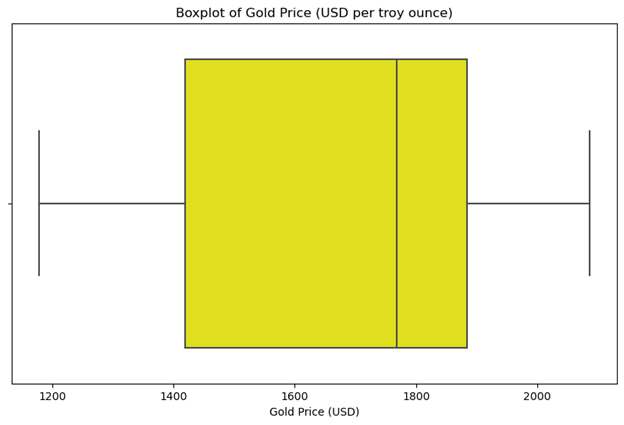
\includegraphics[width=1\textwidth]{bibliography/Figure/boxplot_gold.png}
    \caption{Biểu đồ hộp của giá vàng}
    \label{fig:1}
    \end{minipage}
    \hfill
    \begin{minipage}{0.23\textwidth}
    \centering
    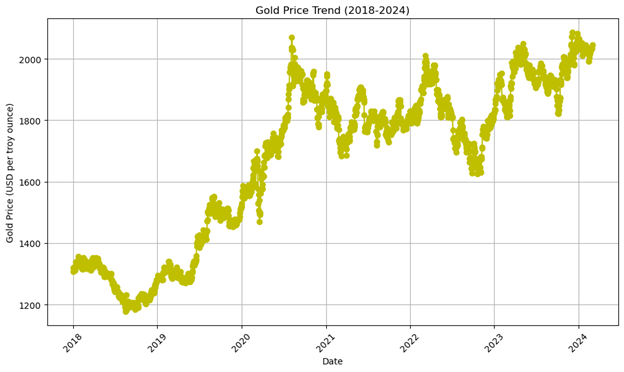
\includegraphics[width=1\textwidth]{bibliography/Figure/line_gold.png}
    \caption{Biểu đồ đường của giá vàng}
    \label{fig:2}
    \end{minipage}
\end{figure}

\begin{figure}[H]
    \centering
    \begin{minipage}{0.23\textwidth}
    \centering
    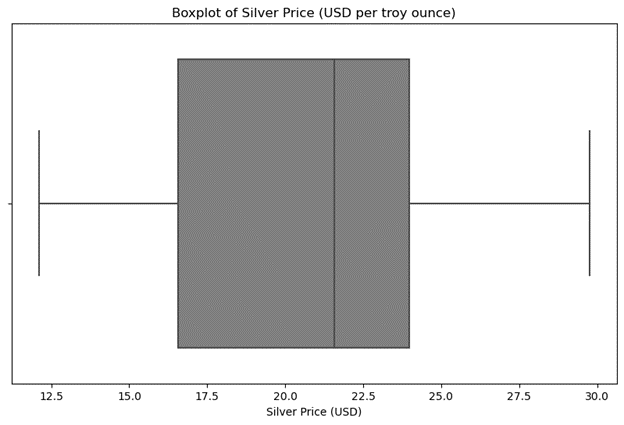
\includegraphics[width=1\textwidth]{bibliography/Figure/boxplot_silver.png}
    \caption{Biểu đồ hộp của giá bạc}
    \label{fig:3}
    \end{minipage}
    \hfill
    \begin{minipage}{0.23\textwidth}
    \centering
    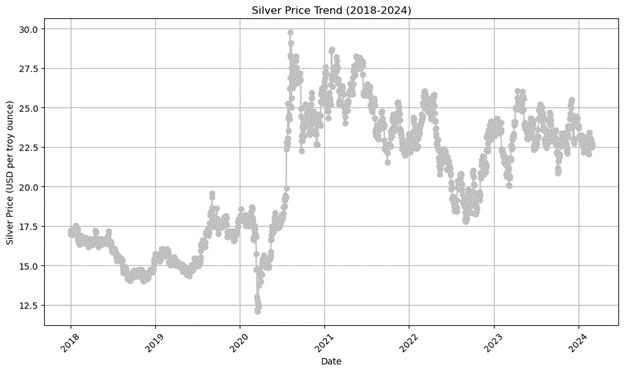
\includegraphics[width=1\textwidth]{bibliography/Figure/line_silver.png}
    \caption{Biểu đồ đường của giá bạc}
    \label{fig:4}
    \end{minipage}
\end{figure}

\begin{figure}[H]
    \centering
    \begin{minipage}{0.23\textwidth}
    \centering
    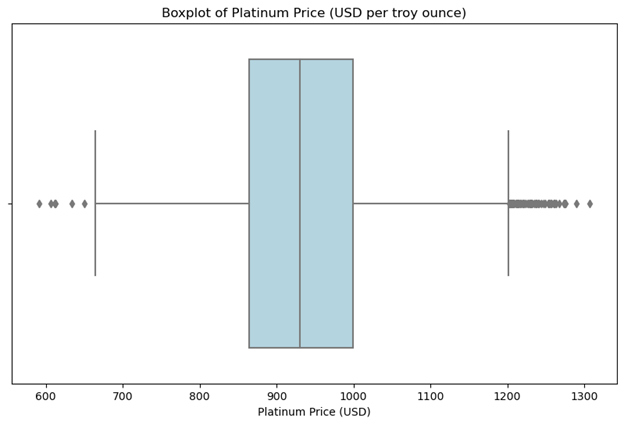
\includegraphics[width=1\textwidth]{bibliography/Figure/boxplot_pt.png}
    \caption{Biểu đồ hộp của giá bạch kim}
    \label{fig:5}
    \end{minipage}
    \hfill
    \begin{minipage}{0.23\textwidth}
    \centering
    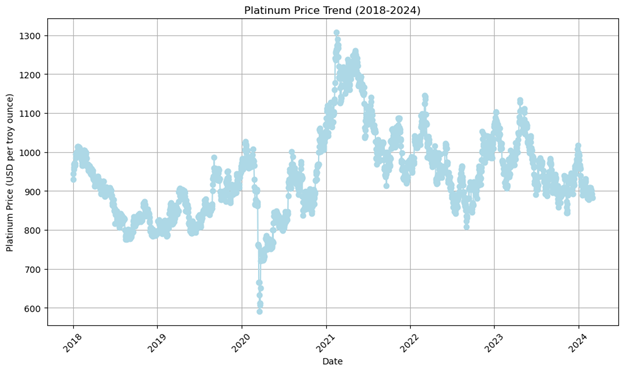
\includegraphics[width=1\textwidth]{bibliography/Figure/line_pt.png}
    \caption{Biểu đồ đường của giá bạch kim}
    \label{fig:6}
    \end{minipage}
\end{figure}




\subsection{Công cụ sử dụng}
Trong quá trình nghiên cứu và phân tích dữ liệu để dự báo giá khoáng sản, nhóm đã sử dụng một số công cụ và thư viện phần mềm phổ biến, chủ yếu được triển khai bằng ngôn ngữ lập trình Python. Danh sách các công cụ và thư viện chính được sử dụng: Pandas, NumPy, Matplotlib, Seaborn, Scikit-learn,... 
\section{Phương pháp}

\subsection{ARIMA}
ARIMA, hay mô hình tự hồi quy tích hợp trung bình chuyển động, là một phương pháp phân tích thống kê sử dụng dữ liệu chuỗi thời gian để hiểu tốt hơn một tập dữ liệu hoặc dự đoán xu hướng tương lai. Nó là một mô hình kết hợp của 2 quá trình tự hồi quy và một trung bình trượt. Dữ liệu quá khứ sẽ được sử dụng để dự đoán dữ liệu trong tương lai.\\
Mô hình ARIMA đại diện cho tự hồi quy tự động (AR), trung bình di chuyển (MA) và tích hợp sai phân (I). \\
\indent\textbullet\ \textbf{Tích hợp (I) d:} Là quá trình sai phân tích hợp, dùng để so sánh sự khác biệt giữa d quan sát.\\
\indent\textbullet\ \textbf{Tự hồi quy (AR) p:} Đây là thành phần tự hồi quy bao gồm tập hợp các trễ của biến hiện tại. Độ trễ bậc p là giá trị quay lại thời điểm p trong quá khứ của chuỗi. Quá trình AR có độ trễ dài hay ngắn phụ thuộc vào tham số trễ p.\\
\indent\textbullet\ \textbf{Trung bình di chuyển (MA) q:} Quá trình trung bình di chuyển (MA) q được hiểu là quá trình thay đổi giá trị trung bình của chuỗi theo thời gian. Quá trình trung bình di chuyển sẽ tìm ra mối liên hệ tuyến tính giữa dữ liệu hiện tại và q lỗi trước đó.

Phương trình hồi quy ARIMA (p, d, q) có thể được biểu diễn như sau:
Phương trình hồi quy tuyến tính đơn giản:
\begin{samepage}
\[\Delta x_t = \sum_{i=1}^{p} \alpha_i \Delta (x_{t-i}) +  \sum_{i=1}^{q} \beta_i \varepsilon_{t-i}\]
\end{samepage}

\subsection{RNN}
Mạng hồi quy RNN (Recurrent Neural Network) là một loại Mạng nơ ron (Neural Network) thường được sử dụng cho dữ liệu tuần tự như chuỗi thời gian. RNN sử dụng đầu ra của bước trước làm đầu vào cho bước hiện tại trong khi Mạng Nơ ron truyền thống tất cả đầu vào và đầu ra đều độc lập với nhau.

Đặc điểm chính và quan trọng nhất của RNN là trạng thái ẩn (Hidden state). Trạng thái này nhớ đầu vào trước đó của mạng. Nó sử dụng cùng trọng số cho đầu vào của mỗi lớp trong mạng.

RNN tính toán trạng thái ẩn ký hiệu là \(h_t\) dựa trên đầu vào hiện tại \(x_t\) và trạng thái ẩn trước đó \(h_{t-1}\):
\[
h_t = \sigma_h (W_{xh} x_t + W_{hh} h_{t-1} + b_h)
\]

Đầu ra \(y_t\) của RNN được tính toán dựa trên trạng thái ẩn hiện tại:
\[
y_t = \sigma_y (W_{hy} h_t + b_o)
\]

Trong đó:
\begin{itemize}
    \item \(\sigma_h, \sigma_y\): Hàm kích hoạt của lớp ẩn và lớp đầu ra.
    \item \(W_{xh}\): Là ma trận trọng số kết nối giữa lớp đầu vào và lớp ẩn.
    \item \(W_{hh}\): Là ma trận trọng số kết nối giữa lớp ẩn và chính nó.
    \item \(W_{hy}\): Là ma trận trọng số kết nối giữa lớp ẩn và lớp đầu ra.
\end{itemize}

Các tham số này được cập nhật bằng cách sử dụng Lan truyền ngược (Backpropagation). Tuy nhiên, do RNN hoạt động trên dữ liệu tuần tự nên nó sẽ sử dụng Backpropagation through Time (BPTT).

Khác với lan truyền ngược truyền thống chỉ tính toán lỗi cho bước đầu ra cuối cùng và cập nhật tham số của mỗi lớp độc lập, BPTT tính toán lỗi cho mỗi bước thời gian trong chuỗi đầu vào, cộng dồn chúng lại và cập nhật tham số của toàn bộ mạng dựa trên lỗi tổng hợp.

\subsection{GRU}
Mạng Neural hồi tiếp nút có cổng (GRU) là một cơ chế cổng trong các mạng nơ ron hồi quy, là một biến thể đơn giản hơn của mạng Bộ nhớ ngắn hạn dài (LSTM). GRU có thể xử lý dữ liệu tuần tự như văn bản, bài viết và chuỗi thời gian.
GRU sử dụng cơ chế cổng để cập nhật có chọn lọc trạng thái ẩn của mạng tại mỗi bước thời gian. Cơ chế cổng được dùng để kiểm soát luồng dữ liệu đi vào và đi ra của mạng. GRU có 2 cơ chế cổng: cổng xóa và cổng cập nhật. \\
Cổng xóa quyết định bao nhiêu phần mà trạng thái trước đây được giữ lại, còn cổng cập nhật quyết định trạng thái ẩn mới có bao nhiêu phần giống trạng thái ẩn cũ. Đầu ra của GRU là tính toán dựa trên số trạng thái ẩn được cập nhật, giúp mô hình có thể ‘nhớ’ thông tin quan trọng từ quá khứ và ‘nhìn’ vào thông tin mới để điều chỉnh trạng thái hiện tại.\\ toán cổng xóa, cổng cập nhật, và số trạng thái ẩn của GRU như sau:\\
Cổng xóa:
\[
R_t = \sigma(X_t W_{xr} + H_{t-1} W_{hr} + b_r)
\]
Cổng cập nhật:
\[
Z_t = \sigma(X_t W_{xz} + H_{t-1} W_{hz} + b_z)
\]
Trong đó:\\
\begin{itemize}
    \item $X_t$: đầu vào ở bước thời gian hiện tại.
    \item $H_{t-1}$: là trạng thái ẩn ở bước trước đó.
    \item $W_{xr}, W_{xz} \in \mathbb{R}^{d \times h}$ và $W_{hr}, W_{hz} \in \mathbb{R}^{h \times h}$: là các trọng số.
    \item $b_r, b_z \in \mathbb{R}^{1 \times h}$: là các tham số độ chênh.
    \item $\sigma$: là hàm sigmoid để 2 giá trị thu được thuộc khoảng $(0,1)$.
\end{itemize}

\vspace{-1em} % Điều chỉnh giá trị này để giảm khoảng cách
\begin{figure}[H]
    \centering
    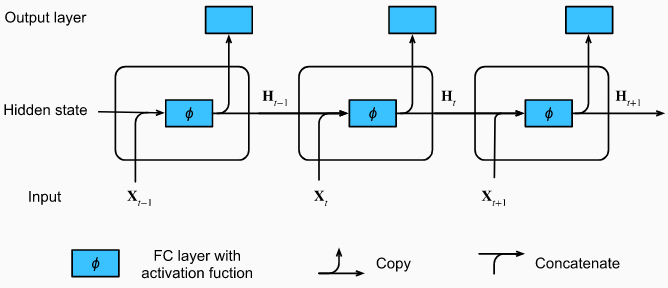
\includegraphics[width=0.5\textwidth]{bibliography/Figure/GRUModel.png}
    \caption{Mô hình GRU}
    \label{fig:GRU_Model}
\end{figure}

\subsection{FFT}
Biến đổi Fourier nhanh (FFT) là một thuật toán cực kì hiệu quả để chuyển đổi một tín hiệu rời rạc miền thời gian sang miền tần số dựa trên biến đổi Fourier rời rạc (DFT). Phép biến đổi DFT phân tích một dãy các số thành các thành phần ở các tần số khác nhau. Phép biến đổi này giúp xác định các thành phần tần số chính của chuỗi thời gian từ đó dự báo các giá trị tương lai dựa trên các thành phần này.

Phép biến đổi Fourier rời rạc - DFT của một tín hiệu rời rạc cho trước \( x_n = [x_0, x_1, \ldots, x_{N-1}] \) được cho bởi biểu thức sau:
\[
X_k = 
\begin{cases} 
\sum_{n=0}^{N-1} x(n) e^{-i \frac{2\pi}{N} kn} & \text{Nếu } 0 \leq k \leq N-1 \\ 
0 & \text{Nếu } k \text{ thuộc phần còn lại} 
\end{cases}
\]
trong đó: \(i\) là đơn vị phức. 

Tính toán biến đổi DFT có độ phức tạp là \(O(N^2)\).

FFT đã được ra đời để khắc phục tốc độ xử lí của DFT. Giả thiết dãy \(x(n)\) có độ dài \(N = 2^i\), nếu không có dạng lũy thừa 2 thì thêm vài mẫu 0 vào sau dãy \(x(n)\). Nguyên tắc cơ bản mà các thuật toán FFT đều dựa vào là phân chia DFT \(N\) mẫu thành các DFT nhỏ hơn một cách liên tục. 

Với \(N = 2^i\), đầu tiên ta sẽ phân chia DFT \(N\) mẫu thành các DFT \(N/2\) mẫu, sau đó phân chia DFT \(N/2\) mẫu thành \(N/4\) mẫu và cứ thế cho đến khi được DFT dài \(N = 2\). Về bản chất nó là đệ quy. Do đó độ phức tạp của FFT được xác định là \(O(N \log_2 (N))\).

Thuật toán FFT:
\[
X(k) = \sum_{n=0}^{\frac{N}{2}-1} x_{2n} e^{-i \frac{2\pi}{N} (2n) k} + \sum_{n=0}^{\frac{N}{2}-1} x_{2n+1} e^{-i \frac{2\pi}{N} (2n+1) k}
\]

\subsection{PatchTST}
PatchTST là mô hình sử dụng Transformer để dự đoán đa biến và học biểu diễn tự giám sát. Dựa trên hai phần chính: \\
\begin{enumerate}
    \item \textbf{Vá dữ liệu (Patching) :} phân đoạn chuỗi thời gian thành các đoạn nhỏ cấp độ chuỗi con, được sử dụng làm các token đầu vào cho Transformer.
    \item \textbf{Kênh truyền độc lập:} mỗi kênh chứa một chuỗi thời gian đơn biến duy nhất, sử dụng cùng trọng số Transformer và trọng số nhúng trên tất cả các chuỗi. 
\end{enumerate}
Kiến trúc mô hình PatchTST sử dụng bộ mã hóa Transformer gốc, mỗi chuỗi đơn biến có độ dài \( L \) được chia thành các mảnh, đưa vào Transformer một cách độc lập, và tạo ra \( T \) giá trị tương lai \( (x_{L+1}, \ldots, x_{L+T}) \).
\begin{figure}[H]
    \centering
    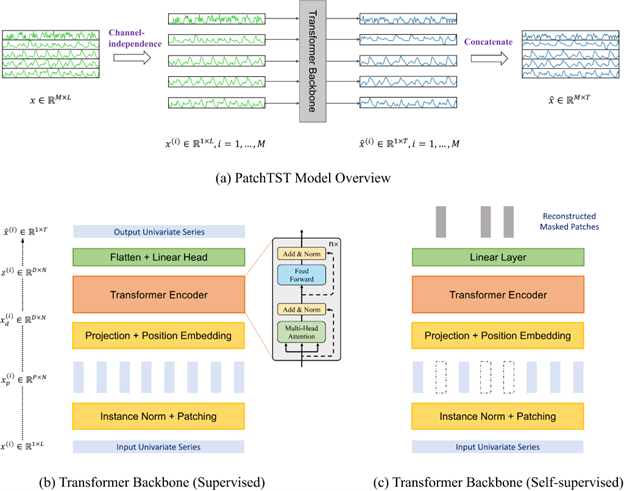
\includegraphics[width=0.5\textwidth]{bibliography/Figure/PatchTSTWorkflow.png}
    \caption{Mô hình PatchTST}
    \label{fig:PatchTST_Model}
\end{figure}
Dữ liệu chuỗi thời gian đa biến \( x \in \mathbb{R}^{M \times L} \) được chia thành các chuỗi đơn biến \( x^{(i)} \in \mathbb{R}^{1 \times L} \) với \( i = 1, \ldots, M \), sau đó được đưa vào Transformer Backbone để xử lý. Các quy trình tiến tới (forward process) là độc lập, và các dự đoán đầu ra \( \hat{x}^{(i)} \in \mathbb{R}^{1 \times T}, i = 1, \ldots, M \) được gộp lại để tạo ra đầu ra cuối cùng \( \hat{x} \in \mathbb{R}^{M \times T} \).

PatchTST có hai biến thể:
\begin{itemize}
    \item \textbf{PatchTST có giám sát:} Sử dụng dữ liệu có nhãn.
    \item \textbf{PatchTST tự giám sát:} Không yêu cầu dữ liệu có nhãn.
\end{itemize}



\subsection{LSTM}
LSTM (Bộ nhớ dài hạn) là một loại mạng nơ-ron hồi quy (RNN) được thiết kế để giải quyết vấn đề gradient biến mất trong các RNN truyền thống. Lợi thế của LSTM là khả năng xử lý khoảng cách xa giữa các thông tin, làm cho nó trở nên hữu ích trong các ứng dụng như nhận dạng giọng nói, dịch máy và phân tích chuỗi thời gian.
\\
Một đơn vị LSTM bao gồm một ô nhớ, một cổng đầu vào, một cổng đầu ra và một cổng quên. Ô nhớ lưu giữ thông tin trong thời gian dài, trong khi các cổng kiểm soát dòng chảy của thông tin vào và ra khỏi ô. Cổng quên quyết định thông tin nào cần bỏ qua, cổng đầu vào quyết định thông tin mới nào cần lưu trữ, và cổng đầu ra quyết định thông tin nào cần xuất ra, giúp mạng LSTM duy trì các phụ thuộc dài hạn hữu ích để đưa ra dự đoán.
\\
Cổng quên xóa thông tin không còn hữu ích khỏi ô nhớ. Phương trình của cổng quên là:\\
\begin{equation*}
    f_t = \sigma(W_f [h_{t-1}, x_t] + b_f)
\end{equation*}

Trong đó:
\begin{itemize}
    \item $\sigma$: Hàm kích hoạt Sigmoid
    \item $W_f$ và $b_f$: Trọng số và độ lệch của cổng quên
\end{itemize}

Cổng đầu vào sẽ thêm thông tin hữu ích vào ô nhớ. Phương trình cho cổng đầu vào là:
\\
\begin{align*}
    i_t &= \sigma(W_i [h_{t-1}, x_t] + b_i) \\
    \tilde{C}_t &= \tanh(W_c [h_{t-1}, x_t] + b_c) \\
    C_t &= f_t \cdot C_{t-1} + i_t \cdot \tilde{C}_t
\end{align*}

Trong đó:
\begin{itemize}
    \item $i_t$: Đầu vào tại thời điểm t
    \item $C_{t-1}$: Ô nhớ tại thời điểm t-1
    \item $W_c, b_c$: Trọng số và độ lệch của ô nhớ
    \item $\tanh$: Hàm kích hoạt Tanh
\end{itemize}

Cổng đầu ra sẽ trích xuất thông tin hữu ích từ ô nhớ hiện tại để trình bày như đầu ra. Phương trình cho cổng đầu ra là:

\begin{equation*}
    o_t = \sigma(W_o [h_{t-1}, x_t] + b_o)
\end{equation*}


\subsection{SES}
Mô hình Smoothing Exponential đơn giản (SES) là một phương pháp dự báo thời gian đơn giản và hiệu quả được sử dụng để làm mịn dữ liệu chuỗi thời gian và dự đoán giá trị trong tương lai. SES đặc biệt hữu ích khi cần dự báo ngắn hạn trên dữ liệu không có xu hướng hoặc mùa vụ rõ rệt. Phương pháp này hoạt động bằng cách áp dụng trọng số giảm một cách mũ màu mực cho các quan sát trước đó, từ đó làm mịn các biến động ngẫu nhiên trong dữ liệu.
\\
Công thức:
\begin{equation}
s_t = \alpha x_t + (1 - \alpha) s_{t-1} + \alpha (x_t - s_{t-1})
\end{equation}

\begin{itemize}
  \item $s_t$: giá trị dự đoán
  \item $s_{t-1}$: giá trị dự đoán trước đó
  \item $\alpha$: hệ số làm mịn $(0 < \alpha < 1)$
  \item $t$: thời điểm
\end{itemize}
Khi giá trị của \( \alpha \) lớn (gần với 1), mức độ làm mịn giảm. Điều này có nghĩa là thuật toán SES sẽ có ít làm mịn hơn và phản ứng mạnh mẽ hơn đối với những thay đổi gần đây nhất trong dữ liệu. Các giá trị dự đoán sẽ gần với các giá trị quan sát gần đây nhất.
\section*{Lời cảm ơn}


Chúng em xin gửi lời cảm ơn chân thành đến Phó Giáo sư Tiến sĩ Nguyễn Đình Thuân và Trợ giảng Nguyễn Minh Nhựt vì sự tận tâm và hướng dẫn nhiệt tình của thầy và anh. Những bài học quý báu từ thầy đã giúp chúng em hoàn thành dự án này và sẽ là nền tảng vững chắc cho những nỗ lực tương lai của chúng em. Dự án này sẽ không thể hoàn thành nếu thiếu sự giám sát và chỉ đạo của thầy.

Trong suốt quá trình thực hiện dự án, chúng em đã gặp không ít khó khăn và thử thách. Nhưng nhờ có sự đoàn kết và hợp tác, chúng em đã vượt qua tất cả và hoàn thành công việc. Dự án này cũng đã mang lại cho chúng em cơ hội thực hành thực tế, giúp chúng em tích lũy được nhiều kinh nghiệm quý báu.

Chúng em cũng xin gửi lời cảm ơn đến các thành viên trong nhóm vì những đóng góp và sự hỗ trợ nhiệt tình trong suốt quá trình thực hiện dự án. Nhờ có sự hỗ trợ và cộng tác của các bạn, chúng em đã học hỏi được nhiều điều và hoàn thành công việc một cách tốt nhất.
\section{Kết quả thực nghiệm}

\subsection{Kết quả thực nghiệm và đánh giá}
% \subsubsection{Dữ liệu giá Vàng}
\begin{figure}[t] 
\subsubsection{Dữ liệu giá Vàng}
    % \centering
    \raggedright
    \begin{minipage}{0.5\textwidth}
        \centering
        \begin{minipage}{0.45\textwidth}
            \centering
            \includegraphics[width=\textwidth]{bibliography/Figure/Linear_gold_8-2.png}
            \caption{Linear Regression tỷ lệ 8:2}
        \end{minipage}
        \hfill
        \begin{minipage}{0.45\textwidth}
            \centering
            \includegraphics[width=\textwidth]{bibliography/Figure/Arima_gold_7-3.png}
            \caption{Mô hình ARIMA tỷ lệ 7:3}
        \end{minipage}
        \hfill
        \begin{minipage}{0.45\textwidth}
            \centering
            \includegraphics[width=\textwidth]{bibliography/Figure/RNN_gold_7-3.png}
            \caption{Mô hình RNN tỷ lệ 7:3}
        \end{minipage}
        \hfill
        \begin{minipage}{0.45\textwidth}
            \centering
            \includegraphics[width=\textwidth]{bibliography/Figure/Gru_gold_7-3.png} 
            \caption{Mô hình GRU tỷ lệ 7:3}
        \end{minipage}
        \hfill
        \begin{minipage}{0.45\textwidth}
            \centering
            \includegraphics[width=\textwidth]{bibliography/Figure/LSTM_gold_7-3.png} 
            \caption{Mô hình LSTM tỷ lệ 7:3}
        \end{minipage}
        \hfill
        \begin{minipage}{0.45\textwidth}
            \centering
            \includegraphics[width=\textwidth]{bibliography/Figure/FFT_gold_8-2.png} 
            \caption{Mô hình FFT tỷ lệ 8:2}
        \end{minipage}
         \hfill
        \begin{minipage}{0.45\textwidth}
            \centering
            \includegraphics[width=\textwidth]{bibliography/Figure/TBATS_gold_8-2.png} 
            \caption{Mô hình TBATS tỷ lệ 8:2}
        \end{minipage}
        \hfill
        \begin{minipage}{0.45\textwidth}
            \centering
            \includegraphics[width=\textwidth]{bibliography/Figure/SES_gold_7-3.png} 
            \caption{Mô hình SES tỷ lệ 7:3}
        \end{minipage}
        \hfill
        \begin{minipage}{0.45\textwidth}
            \centering
            \includegraphics[width=\textwidth]{bibliography/Figure/PatchTST_gold_9-1.png} 
            \caption{Mô hình PatchTST tỷ lệ 9:1}
        \end{minipage}
        \begin{minipage}{0.45\textwidth}
            \centering
            \includegraphics[width=\textwidth]{bibliography/Figure/NHits_gold_8-2.jpg} 
            \caption{Mô hình N-Hits tỷ lệ 8:2}
        \end{minipage}
    \end{minipage}
    \caption{Các mô hình dự đoán giá vàng tốt nhất}
    \label{fig:gold-images}
\end{figure}
% \FloatBarrier
% \subsubsection{Dữ liệu giá Bạc}
% \pagebreak

\begin{thebibliography}{00}
    \bibitem{b1} Tawum Juvert Mbah, Haiwang Ye, Jianhua Zhang & Mei Long,
    Using LSTM and ARIMA to Simulate and Predict Limestone Price Variations (06/01/2021).
    \bibitem{b2} Bojun Yin, Renguang Zuo, Yihui Xiong, Mineral Prospectivity Mapping via Gated Recurrent Unit Model (25/11/2021).
    \bibitem{b3} F.Javier Galán-Sales, Pablo Reina-Jiménez, Manuel Carranza-García, José María Luna-Romera, An Approach to Enhance Time Series Forecasting by Fast Fourier Transform (31/08/2023).
    \bibitem{b4}Improve, A. 27 F. (2018, October 3). Introduction to recurrent neural network. GeeksforGeeks. https://www.geeksforgeeks.org/introduction-to-recurrent-neural-network/
    \bibitem{b5}Gated recurrent unit networks. (2019, July 9). GeeksforGeeks. https://www.geeksforgeeks.org/gated-recurrent-unit-networks/
    \bibitem{b6}De Livera, A. M., Hyndman, R. J., & Snyder, R. D. (n.d.). Forecasting time series with complex seasonal patterns using exponential smoothing. Robjhyndman.com. Retrieved June 20, 2024, from https://robjhyndman.com/papers/ComplexSeasonality.pdf (trang 9, 10, 11, 12)
    \bibitem{b7} VanderPlas, J. (n.d.). Understanding the FFT algorithm. Github.Io. Retrieved June 20, 2024, from https://jakevdp.github.io/blog/2013/08/28/understanding-the-fft/
    \bibitem{b8} Yuqi Nie, Nam h. Nguyen, Phanwadee Sinthong, Jayant Kalagnanam, A Time Series is Worth 64 Words: Long-term Forecasting with Transformers (published 5 Mar 2023).
    \bibitem{b9} Gough, B. (n.d.). FFT Algorithms. Cinvestav.Mx. Retrieved June 20, 2024, from https://www.tamps.cinvestav.mx/~wgomez/material/AID/fft_algorithms.pdf
    
    \end{thebibliography}
    \vspace{12pt}

